As estratégias propostas, ATU (agnóstica baseada em densidade) e HTU (híbrida baseada em densidade), a adaptação para multiclasse SGmulti e aquelas implementadas conforme a literatura, tiveram seu desempenho
geral % preditivo e de variabilidade
comparado visualmente por meio de curvas de ranqueamento.
As diferenças estatisticamente significativas foram reveladas pelo teste de Friedman com teste post-hoc de Nemenyi (Capítulo \ref{metodologia}).
A avaliação no nível base é dividida nas seguintes seções: desempenho preditivo (Seção \ref{despred}), variabilidade (Seção \ref{variab}) e custo computacional (Seção \ref{cuscomp}).
Adicionalmente, na Seção \ref{poralg}, uma análise separada por algoritmos de aprendizado é realizada.
Por fim, na Seção \ref{desmetap}, o meta-aprendiz é situado no contexto do nível base de forma a conduzir aos experimentos no nível meta, das macrosseções posteriores \ref{expmeta} e \ref{outmod}.

\subsection{Acurácia preditiva}\label{despred}
As curvas de ranqueamento das estratégias EERent\footnote{baseada no erro esperado}, HTUeuc, ATUeuc, TUeuc\footnote{baseada em densidade que considera exemplos rotulados}, Mar\footnote{baseada na margem de incerteza}, SGmulti\footnote{proposta multiclasse de busca no espaço de hipóteses}, HS\footnote{baseada em agrupamento hierárquico}, Rnd\footnote{amostragem aleatória} e DWeuc\footnote{baseada em densidade sem considerar exemplos rotulados} são exibidas na Figura \ref{curvasrank} - toda a coleção de conjuntos de dados foi utilizada.
\begin{figure}
	\centering
	\includestandalone[mode=buildmissing]{figrankmedio}
	\caption[Curvas de ranqueamento ($\mu_{\kappa}$).]{Curvas de ranqueamento. Medida comparada: $\mu_{\kappa}$. \textit{As siglas das estratégias propostas estão grafadas em negrito e a estratégia adaptada para multiclasse em itálico. A média considera quatro algoritmos e noventa conjuntos de dados.}}
	\label{curvasrank}
\end{figure}
As propostas ATUeuc e HTUeuc compartilham, juntamente com EERent, o topo do gráfico com colocações acima de 4,5 em praticamente todo o período experimental.
Exceto por TUeuc, as demais estratégias, inclusive SGmulti, se mantiveram abaixo do ranqueamento médio (5\textordfeminine\xspace colocação).
Logo, as duas propostas se mostraram competitivas, enquanto que a estratégia adaptada para multiclasse obteve um desempenho abaixo da média.
Por outro lado, o bom desempenho em geral, e especialmente a predominância de EERent nas primeiras 10 consultas, pode ser resultado dela ser a única estratégia que requereu, antes de cada consulta, a subamostragem de 100 exemplos explicada previamente na Seção \ref{eerconfig}.
Essa subamostragem tem, incidentalmente, um efeito exploratório, pois introduz (pseudo)aleatoriedade numa estratégia que, de outra forma, seria determinística.

HTUeuc e ATUeuc superam EERent visualmente durante a maior parte da primeira metade das consultas.
Entretanto, após aproximadamente 55 consultas, elas apresentam uma baixa gradual em sua posição no gráfico.
%reduzem sua colocação gradativamente.
Esse efeito é mais intenso para a estratégia ATUeuc - conforme esperado.
Tal constatação é compatível com a expectativa de que um viés de amostragem exploratório deixe de ser vantajoso após o trecho inicial do aprendizado.
O mesmo efeito pode ser notado nas outras estratégias agnósticas, HS, SGmulti e Rnd.
Elas cedem posições para as estratégias prospectivas com o decorrer do aprendizado.
De forma correspondente, as curvas de estratégias prospectivas, como TUeuc e Mar, apresentam uma trajetória ascendente conforme aumenta a quantidade de consultas realizadas.
Por fim, o destaque negativo foi DWeuc, demonstrando que a ponderação pela densidade pode ser bastante prejudicial em alguns casos.
A diferença entre TU (incluindo sucessoras, ATU e HTU) e DW é que a primeira assegura o afastamento do grupo de exemplos rotulados.
O afastamento ocorre por meio da inversa ponderação pela densidade desse grupo de exemplos.

Quando considerada a ALC (\textit{Area Under the Learning Curve} - Capítulo \ref{metodologia}), não foram detectadas diferenças estatisticamente significativas entre EERent, HTUeuc e ATUeuc - conforme ilustra a Tabela \ref{friedmedio}.
\input tex/friedmedio
Entretanto, alguns pontos podem ser destacados acerca das propostas com diferenças estatisticamente significativas ($\alpha=0,01$) - listados a seguir.
\begin{itemize}
   \item ATUeuc superou todas as outras estratégias agnósticas.
   \item ATUeuc e HTUeuc superaram sua antecessora comum, TUeuc.
   \item Ambas também superaram Mar, SGmulti e DWeuc.
   \item Embora SGmulti tenha superado significativamente apenas a pior estratégia (DWeuc), ela obteve o menor número de derrotas para Rnd, provavelmente por selecionar aleatoriamente exemplos da região de desacordo. Isso está de acordo com a expectativa de que as vantagens de um maior enviesamento em alguns domínios está associada a desvantagens em outros domínios.
   \item Enquanto nenhuma das outras estratégias empataram com Rnd (Anexo \ref{anresdet}), SGmulti empatou 112 vezes, devido à sua semelhança com Rnd - conforme contagem na Tabela \ref{contamedio}.
   \item HTUeuc obteve 8 últimas colocações - a menor quantidade de ocorrências dentre as estratégias sob comparação.
\end{itemize}
Com relação ao patente mau desempenho apresentado na curva de DWeuc, pode-se atribuí-lo à grande quantidade de derrotas para Rnd (242).
Entretanto, DWeuc obteve o quarto maior número de primeiras colocações, indicando que uma estratégia de amostragem pode ser positivamente enviesada para alguns conjuntos de dados/algoritmos e negativamente enviesada para muitos outros, em conformidade com o teorema NFL aplicado ao aprendizado ativo (\textit{No Free Lunch} - Seção \ref{hipoteses}).

% 360 pares conjunto-algoritmo
Um indicativo da viabilidade do aprendizado ativo em geral é que a amostragem aleatória (Rnd) teve o menor número de primeiros lugares e venceu as demais estratégias (exceto DWeuc e Mar) menos vezes do que perdeu.
Isto é, a maioria dos valores da coluna \textit{derrotas para Rnd} está abaixo de 180, que é a metade do total de pares conjunto-algoritmo testados.
Ainda confirmando a efetividade do aprendizado ativo, HS superou a amostragem aleatória, respeitando, assim, a garantia teórica fornecida pelo seu autor.

Finalmente, há uma limitação nessa avaliação baseada apenas na contagem dos primeiros colocados.
Ela ignora estratégias bem posicionadas que não tenham atingido o maior valor da medida de desempenho, mesmo que a diferença para a primeira colocação seja diminuta.
Na prática, uma estratégia frequentemente bem colocada é preferível a uma estratégia frequentemente mal colocada que tenha fortuitamente o maior número de primeiras colocações.
Portanto, optou-se por apresentar, adicionalmente, uma contagem de vitórias que considerasse os três melhores colocados.
É possível verificar na Tabela \ref{tabwin3} que HTUeuc, seguida de ATUeuc, se torna preferível a EERent segundo a nova forma de contagem.
Além disso, HTUeuc mantém o melhor número de ocorrências entre as três últimas colocações.
\begin{table}
\caption[Contagem das três melhores e três piores colocações (ALC-$\mu_{\kappa}$).]{Contagem das três melhores e três piores colocações. Medida: ALC-$\mu_{\kappa}$. \textit{Detalhes na Tabela \ref{exfried}.}}
\label{tabwin3}
\centering
\scalebox{0.82}{
\begin{tabular}{lccc}
\toprule             
		\textbf{Estratégia} & \makecell{\textbf{Primeiras }\\\textbf{colocações}} & \makecell{\textbf{Derrotas} \\ \textbf{para Rnd}}  & \makecell{\textbf{Últimas}\\\textbf{colocações}} \\
\midrule
\textbf{HTUeuc}     & \bom{197} & 109 & \bom{61} \\
\textbf{ATUeuc}     & \bomd{190} & 96 & 74 \\
EERent     & 189 & \bomd{92} & \bomd{65} \\
TUeuc      & 131 & 148 & 113 \\
HS        & 95 & 129 & 95 \\
Mar        & 80 & 187 & 172 \\
\textit{SGmulti}    & 75 & \bom{88} & 127 \\
DWeuc      & 73 & \ruim{242} & \ruim{227} \\
Rnd        & \ruim{66} & - & 165 \\
\bottomrule
\end{tabular}
}
\end{table}
Consequentemente, pode-se afirmar que, para a coleção, estratégias e algoritmos empregados \destaque{HTUeuc é a estratégia mais segura em termos de consistência/regularidade, pois frequentemente está entre as melhores e raramente está entre as piores}.

Outro aspecto da qualidade de uma estratégia de amostragem ativa é a estabilidade de seu desempenho.
Os resultados relativos à estabilidade são reportados a seguir, na Seção \ref{variab}, por meio do desvio padrão do valor da medida de desempenho preditivo ($\sigma_{\kappa}$).

\subsection{Variabilidade}\label{variab}
Uma estratégia estável deve ser pouco sensível a variações na constituição da reserva de exemplos.
Uma grande variabilidade coloca o orçamento sob o risco de ser gasto sem que seja atingido um desempenho adequado e pode levar a custos excedentes de rotulação imprevisíveis.
Assim, analisar a estabilidade das estratégias tem fundamental importância na escolha de estratégias.
% Uma aplicação real tem custos de rotulação irreversíveis que impossibilitam a experimentação de mais de uma estratégia.
A medida aqui adotada para verificar a variabilidade de desempenho das estratégias é baseada em $\sigma_{\kappa}$, analogamente aos resultados anteriores, baseados em $\mu_{\kappa}$.
A Figura \ref{curvasrisco} contém as curvas de valores $\sigma_{\kappa}$.
\begin{figure}
	\centering
	\includestandalone[mode=buildmissing]{figmediorisco}
	\caption{Curvas representando a variabilidade das estratégias.}
	\label{curvasrisco}
\end{figure}

Cada estratégia começou com $\sigma_{\kappa}$ abaixo do valor de pico da curva, possivelmente devido à constante presença inicial de um rótulo por classe em todas as 25 reservas da validação cruzada.
A partir da vigésima consulta, todas as estratégias passaram a apresentar valores descendentes.
Elas se tornavam mais estáveis com o crescimento do conjunto de treinamento.
%crescia.
Portanto, pode-se supor que a escolha de estratégias mais estáveis é prioritária em orçamentos mais restritos.
Os mesmos resultados são apresentados em termos relativos na Figura \ref{curvasrankrisco}, por meio das curvas de ranqueamento baseadas nos valores de $\sigma_{\kappa}$.
\begin{figure}
	\centering
	\includestandalone[mode=buildmissing]{figrankmediorisco}
	\caption[Curvas de ranqueamento ($\sigma_{\kappa}$).]{Curvas de ranqueamento. Medida comparada: $\sigma_{\kappa}$. \textit{A colocação média é calculada ao longo de toda a coleção e para os quatro algoritmos de aprendizado.}}
	\label{curvasrankrisco}
\end{figure}

As curvas ranqueadas de ATUeuc e HTUeuc atingiram as melhores colocações na primeira metade das consultas e foram similares a EERent na segunda metade.
Conforme ilustra a Tabela \ref{friedmediorisco}, é possível atestar com diferenças estatisticamente significativas ($\alpha=0,01$) que, para a coleção de conjuntos de dados, estratégias e algoritmos de aprendizado empregados,
\destaque{ATUeuc e HTUeuc têm a menor variabilidade.}

\input tex/friedmediorisco

DWeuc obteve o segundo maior número de primeiras colocações, porém também obteve a maior quantidade de últimas colocações - conforme mostrado na Tabela \ref{contamediorisco}.
Uma desvantagem adicional de EERent é seu elevado
%elevada complexidade com relação ao 
custo computacional entre consultas.
Os custos computacional e de esforço humano são discutidos e avaliados na Seção \ref{cuscomp}.

\subsection{Custo}\label{cuscomp}

Idealmente, o tempo requerido por uma estratégia para escolher o próximo exemplo a ser consultado nunca deveria ultrapassar o \textit{tempo de espera tolerável} \cite{conf/amcis/Nah03} por um oráculo humano.
As consequências vão desde o aumento no consumo do tempo de disponibilidade humana até a redução na confiabilidade do processo de supervisão.

A capacidade humana de processamento de informação pode ser afetada por interferências na memória de curto prazo.
De acordo com \citeonline{conf/afips/Miller68}, um exemplo de interferência é a imposição de um período de espera superior a $2s$.
Um período de espera inferior a $1s$ permite que o usuário mantenha o fluxo de pensamento ininterrupto \cite{conf/amcis/Nah03}.
Na Figura \ref{tempos}, a duração média dos períodos de espera mais longos é apresentada para ATUeuc, HTUeuc e EERent.
Note-se que EERent foi diretamente beneficiada pela realização da subamostragem que reduziu a reserva para 100 exemplos (Seção \ref{eerconfig}) - os dez maiores conjuntos de dados da coleção, por exemplo, têm mais de 5000 exemplos e tornariam o experimento computacionalmente inviável para EER.
\begin{figure}
	\centering
	\includestandalone[mode=buildmissing]{tempos}
	\caption[Média de duração das consultas.]{Média de duração das consultas com os maiores períodos de espera de cada execução do procedimento de validação.}
	\label{tempos}
\end{figure}

Naturalmente, a curva de ATUeuc situa-se sempre abaixo da curva de HTUeuc, devido à dispensa do aprendiz por parte daquela.
Contudo, HTU ultrapassou o limite menos crítico ($1s$) em apenas seis conjuntos de dados, mantendo-se abaixo de $5s$ em toda a coleção.
Logo, ambas mostraram-se de baixo impacto do ponto de vista de esforço humano.
As esperas geradas por EERent, por sua vez, atingiram durações superiores ao limite crítico ($2s$) em todos os conjuntos de dados e ultrapassaram $100s$ em seis deles.
% % Miller (1968) argued for the 2-second rule based on the theory of limitations in human short-
% % term memory. According to Miller, short-term memory plays a critical role in human information
% % processing; interference with short-term memory can occur when an individual senses an awareness of
% % waiting after approximately 2 seconds. Thus, to stay uninterrupted in information processing, the 2-
% % second guideline is recommended. For tasks where uninterrupted focus is critical, Nielsen (1995)
% % suggests that computer response should be kept within one second.
% % 
% % 
% % From this study, we found that Web users expect a response in about 2 seconds for simple
% % information retrieval tasks on the Web.
% % A 2-second response is needed to ensure 'smooth' interactions
% % between the WWW and the users.  The findings from this
% % study also suggest that the upper bound for Web users' TWT is 15 seconds when
% % the system does not provide any indication or feedback concerning
% % the download

Assim, apesar do bom desempenho preditivo, EERent pode aumentar o custo com recursos humanos ou mesmo se tornar inviável com certos conjuntos de dados e algoritmos.
Em oposição, estratégias com menor ordem de complexidade reduzem o tempo entre consultas em várias ordens de magnitude.
Logo, dentre as três estratégias com melhor desempenho preditivo,
\destaque{ATUeuc e HTUeuc são consideravelmente mais apropriadas com relação ao custo computacional entre consultas e, consequentemente, de esforço humano.}



\subsection{Acurácia preditiva por algoritmo}\label{poralg}

Os resultados apresentados nas seções anteriores são provenientes de um cenário que permite avaliar o desempenho das estratégias de amostragem ativa sem fazer distinção entre os algoritmos de aprendizado.
Entretanto, é possível que alguns algoritmos sejam intrinsecamente inadequados para certas estratégias.
O especialista em aprendizado de máquina, ciente dessa possibilidade, poderia evitar determinadas combinações.

Do ponto de vista experimental, combinações estratégia-algoritmo inadequadas prejudicam a colocação média no ranqueamento, rebaixando estratégias que, de outra forma, poderiam se posicionar entre as melhores.
De fato, quando é construída uma árvore de decisão para organizar as estratégias de acordo com seu desempenho em todos os pares conjunto-algoritmo, o algoritmo de aprendizado surge como condição primária; ele é a condição do nó raiz - conforme Figura \ref{treebadst}.
A árvore foi induzida pelo algoritmo C4.5w com poda de pelo menos 150 exemplos por folha.
\begin{figure}
	\centering
	\includestandalone[mode=buildmissing]{treeALCKappaperd}
	\caption[Possíveis nichos de inadequação conjunto-estratégia-algoritmo.]{Possíveis nichos de inadequação conjunto-estratégia-algoritmo. Contagem de ocorrências na última colocação.}
	\label{treebadst}
\end{figure}

Cada nó folha contém a contagem de derrotas de cada algoritmo de acordo com a ALC-$\mu_\kappa$.
Os atributos considerados foram: \textit{quantidade de classes, quantidade de atributos, quantidade de exemplos, razão entre quantidade de exemplos e de atributos, percentual de atributos nominais, percentual de exemplos correspondente à classe majoritária, percentual de exemplos correspondente à classe minoritária, razão entre percentual correspondente à classe majoritária e correspondente à classe minoritária e algoritmo de aprendizado}.
% entropia da distr. de classes, orçamento ($\cent\leq 50$ ou $\cent maiorque 50$)
% atributo aceito" {"numérico","nominal","ambos"}
% fronteira" {"rígida","flexível","nenhuma"}
% \afterpage{\clearpage\begin{landscape}

Apesar das variantes de DW serem destaque negativo em praticamente todas as folhas, é possível notar indícios de inadequação entre algoritmos e estratégias.
Por exemplo, EERent poderia ser, de acordo com a árvore, inadequada para C4.5w, 5NNw ou NB com atributos nominais, enquanto que poderia ser adequada nos demais caminhos, dado que não aparece entre as menos adequadas em nenhuma das outras folhas.

Observação similar poderia ser feita para as propostas baseadas em densidade ou para HS, por exemplo.
Logo, uma análise separada por algoritmo mostra-se relevante para limitar a influência das inadequações estratégia-algoritmo na comparação de desempenhos.

Na Figura \ref{curvasrankbands}, é exibida a curva ranqueada da melhor estratégia para cada algoritmo de aprendizado.
\begin{figure}
	\centering
	\includestandalone[mode=buildmissing]{bands}
	\caption[Curvas de ranqueamento ($\mu_{\kappa}$).]{Curvas de ranqueamento. Medida comparada: $\mu_{\kappa}$. \textit{Detalhes na Figura \ref{ilustrafaixas}.} \textit{Cada faixa contém, implicitamente, as curvas de todas as estratégias.}}
	\label{curvasrankbands}
\end{figure}
No início do aprendizado, o comportamento de cada algoritmo foi distinto - conforme evidenciado pelas faixas coloridas que indicam os limites atingidos pelas estratégias.
Próximo ao final da curva, após 60 consultas, a faixa de estratégias correspondente ao algoritmo SVM começa a se destacar, indicando a existência de uma relação entre o desempenho do algoritmo e o instante do aprendizado.

A melhor estratégia variou conforme o algoritmo: EERent foi a melhor para SVM e NB, enquanto que HTUeuc e ATUeuc foram as melhores para C4.5w e 5NNw, respectivamente.
A Figura \ref{separadas} apresenta as faixas 5NN, C4.5w, NB e SVM separadamente, explicitando as curvas de todas as estratégias.
\begin{figure}
\centering
	\includestandalone[mode=buildmissing]{bands5nn}
	\includestandalone[mode=buildmissing]{bandsc45}
	\includestandalone[mode=buildmissing]{bandsnb}
	\includestandalone[mode=buildmissing]{bandsrbf}
\caption[Curvas de ranqueamento por algoritmo de aprendizado ($\mu_{\kappa}$).]{Curvas de ranqueamento separadas por algoritmo de aprendizado. Medida comparada: $\mu_{\kappa}$. \textit{Detalhes na Figura \ref{ilustrafaixas}.}}
\label{separadas}
\end{figure}
Em geral, ATUeuc, HTUeuc e EERent permanecem como as melhores opções com exceção de alguns casos.
SGmulti, por exemplo, se desvinculou positivamente de Rnd com os algoritmos C4.5w e NB e chegou a figurar entre as duas melhores estratégias na segunda metade das consultas com NB.

% começa a falar do que motiva o meta
Dada a diversidade de estratégias, seria esperada uma grande intersecção entre todas as faixas da Figura \ref{curvasrankbands}, apresentada previamente.
Entretanto, a existência de amplas regiões sem intersecção sugere uma predominância do algoritmo de aprendizado na determinação do desempenho do par estratégia-algoritmo.
% O mesmo efeito pode ser observado na amostragem aleatória, dado que está contida em cada faixa.
Consequentemente, seria proveitoso o especialista em aprendizado de máquina dispor de um guia análogo à árvore de decisão da Figura \ref{treebadst} que auxilie na escolha do algoritmo, dada a estratégia; ou, na escolha da estratégia, dado o algoritmo.
Assim, uma possível árvore guia para a escolha manual do par estratégia-algoritmo é apresentada na Figura \ref{treegoodst}.
\begin{figure}
	\centering
	\includestandalone[mode=buildmissing]{treeALCKappa}
	\caption[Possíveis nichos de adequação conjunto-estratégia-algoritmo.]{Possíveis nichos de adequação conjunto-estratégia-algoritmo. Contagem de ocorrências entre as três melhores colocações.}
	\label{treegoodst}
\end{figure}

É possível notar que a distribuição de vitórias muda consideravelmente em cada caminho.
Essa característica é a base do sistema automático de recomendação de algoritmos proposto, cujo meta-aprendiz resultante é comparado no cenário de aprendizado ativo com os demais algoritmos, a seguir, na Seção \ref{desmetap}.

\newpage
\subsection{Acurácia preditiva com meta-aprendiz}\label{desmetap}
Conforme discutido previamente no Capítulo \ref{intro}, o especialista frequentemente não dispõe dos recursos necessários para determinar o melhor algoritmo de aprendizado no cenário de aprendizado ativo.
Por exemplo, a ausência de um conjunto de treinamento suficientemente grande e o desconhecimento dos efeitos da combinação de uma dada estratégia com um dado conjunto de dados aumentam o risco de uma escolha inadequada.
O aprendizado meta-ativo proposto visa reduzir esse risco e tornar menos subjetiva a definição das partes de um sistema de aprendizado ativo.
\textbf{No presente experimento e nos seguintes, o processo de rotulação foi considerado como dois períodos de consultas que correspondem às suas metades.
Isso permitiu que o meta-aprendiz pudesse reconsiderar, após 50 consultas, sua escolha de algoritmo.}

A Figura \ref{curvasrankbandsmeta} contém a faixa de curvas de ranqueamento do meta-aprendiz (metaPCT) comparada às duas faixas de maior destaque no experimento anterior, 5NN e SVM.
O experimento é análogo ao anterior: cada faixa contém as curvas de todas as estratégias.
Consequentemente, o meta-aprendiz fez uma recomendação para cada estratégia e cada período de consultas.
\begin{figure}[]
\centering
	\includestandalone[mode=buildmissing]{bandsmeta}
	\caption[Curvas de ranqueamento com faixas - incluindo meta-aprendiz.]{Curvas de ranqueamento com faixas - incluindo meta-aprendiz. Medida comparada: $\mu_{\kappa}$. Referência: meta-aprendiz baseado na predição do ranqueamento médio - \textit{MetaDef}. \textit{Detalhes na Figura \ref{curvasrankbands}.}}
	\label{curvasrankbandsmeta}
\end{figure}

A faixa metaPCT está visualmente melhor posicionada que as demais em praticamente todo o intervalo de consultas.
A estratégia que tirou maior proveito do meta-aprendiz foi HTUeuc.
Ela superou os pares estratégia-algoritmo ATUeuc-5NN e EERent-SVM, outrora vencedores.
Por outro lado, o melhor par contendo o meta-aprendiz referência (HTUeuc-metaDef) foi equivalente ou inferior a eles.
Essa superioridade de metaPCT em relação à referência indica que o sistema de meta-aprendizado foi efetivamente capaz de extrair conhecimento da coleção.
A significância estatística $\alpha$ das diferenças observadas é confirmada na Figura \ref{alcmeta} para todas as estratégias, exceto SGmulti.
\begin{figure}
\centering
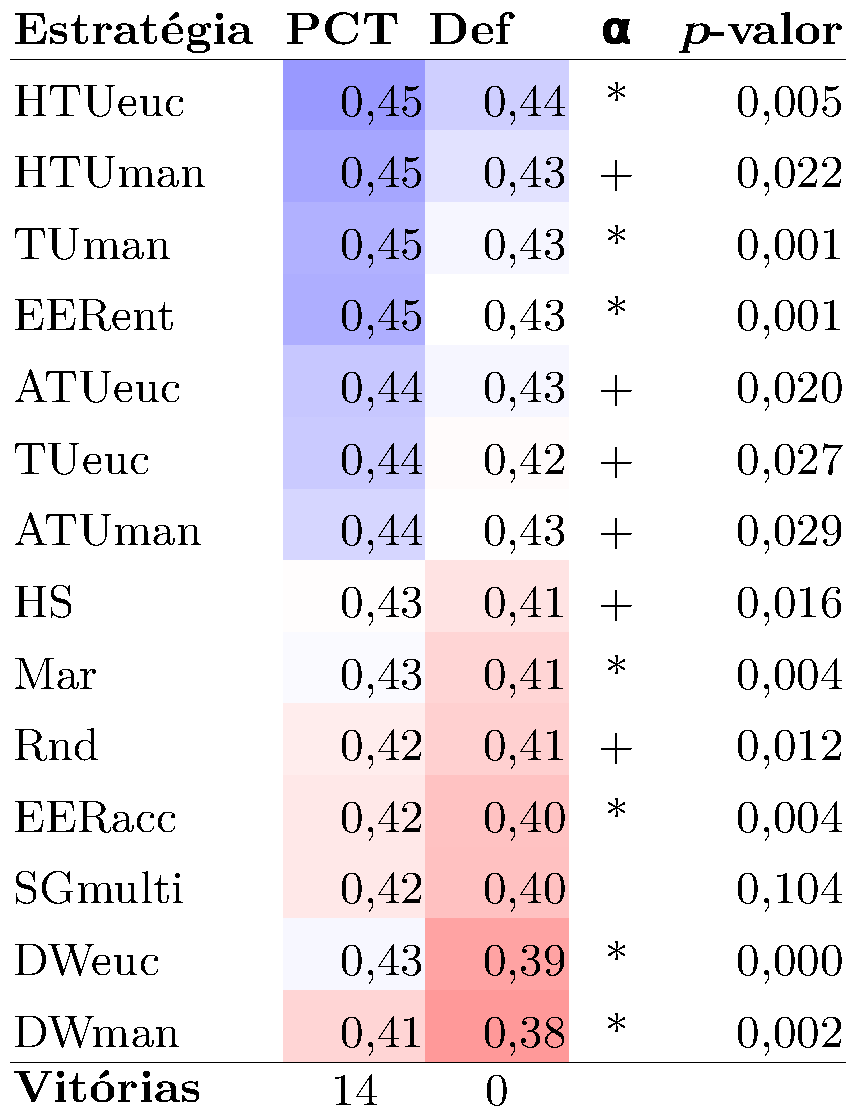
\includegraphics[scale=0.4]{images/metaalc.pdf}
\caption[Comparação de valores de ALC-$\mu_{\kappa}$ obtidos com meta-aprendizes.]{Comparação de valores de ALC-$\mu_{\kappa}$ obtidos com meta-aprendizes.
\textit{Legenda na Tabela \ref{exfried}. Obs.: uma quantidade expressiva de vitórias não significa que os resultados possam ser generalizados a outras coleções, pois todas as linhas são altamente correlacionadas entre si.}}
\label{alcmeta}
% Wilcoxon.scala
% List(, 	Wilcoxon signed rank test with continuity correction, , data:  x and y, V = 2628, p-value = 0.01961, alternative hypothesis: true location shift is not equal to 0) <- log)
% List(, 	Wilcoxon signed rank test with continuity correction, , data:  x and y, V = 2589, p-value = 0.02949, alternative hypothesis: true location shift is not equal to 0) <- log)
% List(, 	Wilcoxon signed rank test with continuity correction, , data:  x and y, V = 2770, p-value = 0.003671, alternative hypothesis: true location shift is not equal to 0) <- log)
% List(, 	Wilcoxon signed rank test with continuity correction, , data:  x and y, V = 2857, p-value = 0.001133, alternative hypothesis: true location shift is not equal to 0) <- log)
% List(, 	Wilcoxon signed rank test with continuity correction, , data:  x and y, V = 2646, p-value = 0.01612, alternative hypothesis: true location shift is not equal to 0) <- log)
% List(, 	Wilcoxon signed rank test with continuity correction, , data:  x and y, V = 2693, p-value = 0.004758, alternative hypothesis: true location shift is not equal to 0) <- log)
% List(, 	Wilcoxon signed rank test with continuity correction, , data:  x and y, V = 2617, p-value = 0.02205, alternative hypothesis: true location shift is not equal to 0) <- log)
% List(, 	Wilcoxon signed rank test with continuity correction, , data:  x and y, V = 2766, p-value = 0.003865, alternative hypothesis: true location shift is not equal to 0) <- log)
% List(, 	Wilcoxon signed rank test with continuity correction, , data:  x and y, V = 2674, p-value = 0.01177, alternative hypothesis: true location shift is not equal to 0) <- log)
% List(, 	Wilcoxon signed rank test with continuity correction, , data:  x and y, V = 1913, p-value = 0.1042, alternative hypothesis: true location shift is not equal to 0) <- log)
% List(, 	Wilcoxon signed rank test with continuity correction, , data:  x and y, V = 2597, p-value = 0.02717, alternative hypothesis: true location shift is not equal to 0) <- log)
% List(, 	Wilcoxon signed rank test with continuity correction, , data:  x and y, V = 2862, p-value = 0.001056, alternative hypothesis: true location shift is not equal to 0) <- log)
% List(, 	Wilcoxon signed rank test with continuity correction, , data:  x and y, V = 1712, p-value = 7.1e-06, alternative hypothesis: true location shift is not equal to 0) <- log)
% List(, 	Wilcoxon signed rank test with continuity correction, , data:  x and y, V = 1462, p-value = 0.001905, alternative hypothesis: true location shift is not equal to 0) <- log)
\end{figure}


Assim, é possível afirmar que, para a coleção, estratégias de amostragem ativa e algoritmos de aprendizado empregados
\destaque{a curva de aprendizado resultante de algoritmos de aprendizado recomendados automaticamente corresponde a um melhor desempenho preditivo do que a curva produzida por um algoritmo fixo, mesmo que o desempenho deste seja predominante na maioria dos conjuntos de dados da coleção - desde que a coleção contenha mais do que um conjunto de um mesmo domínio} (conforme demonstrado posteriormente no Apêndice \ref{apflu}).

Outros algoritmos de aprendizado também podem ser empregados como meta-aprendizes.
Essa possibilidade é avaliada juntamente com os experimentos no nível meta, na Seção \ref{expmeta}.

% \ano{caso possível e se parecer necessário, depois de terminada a tese, indicar se faltou muito pra atingir acurácia passiva, comparando com o kappa da última consulta}